\begin{appendices}
\section{Mind map of elements of Music}
\begin{figure}[h]
\centering
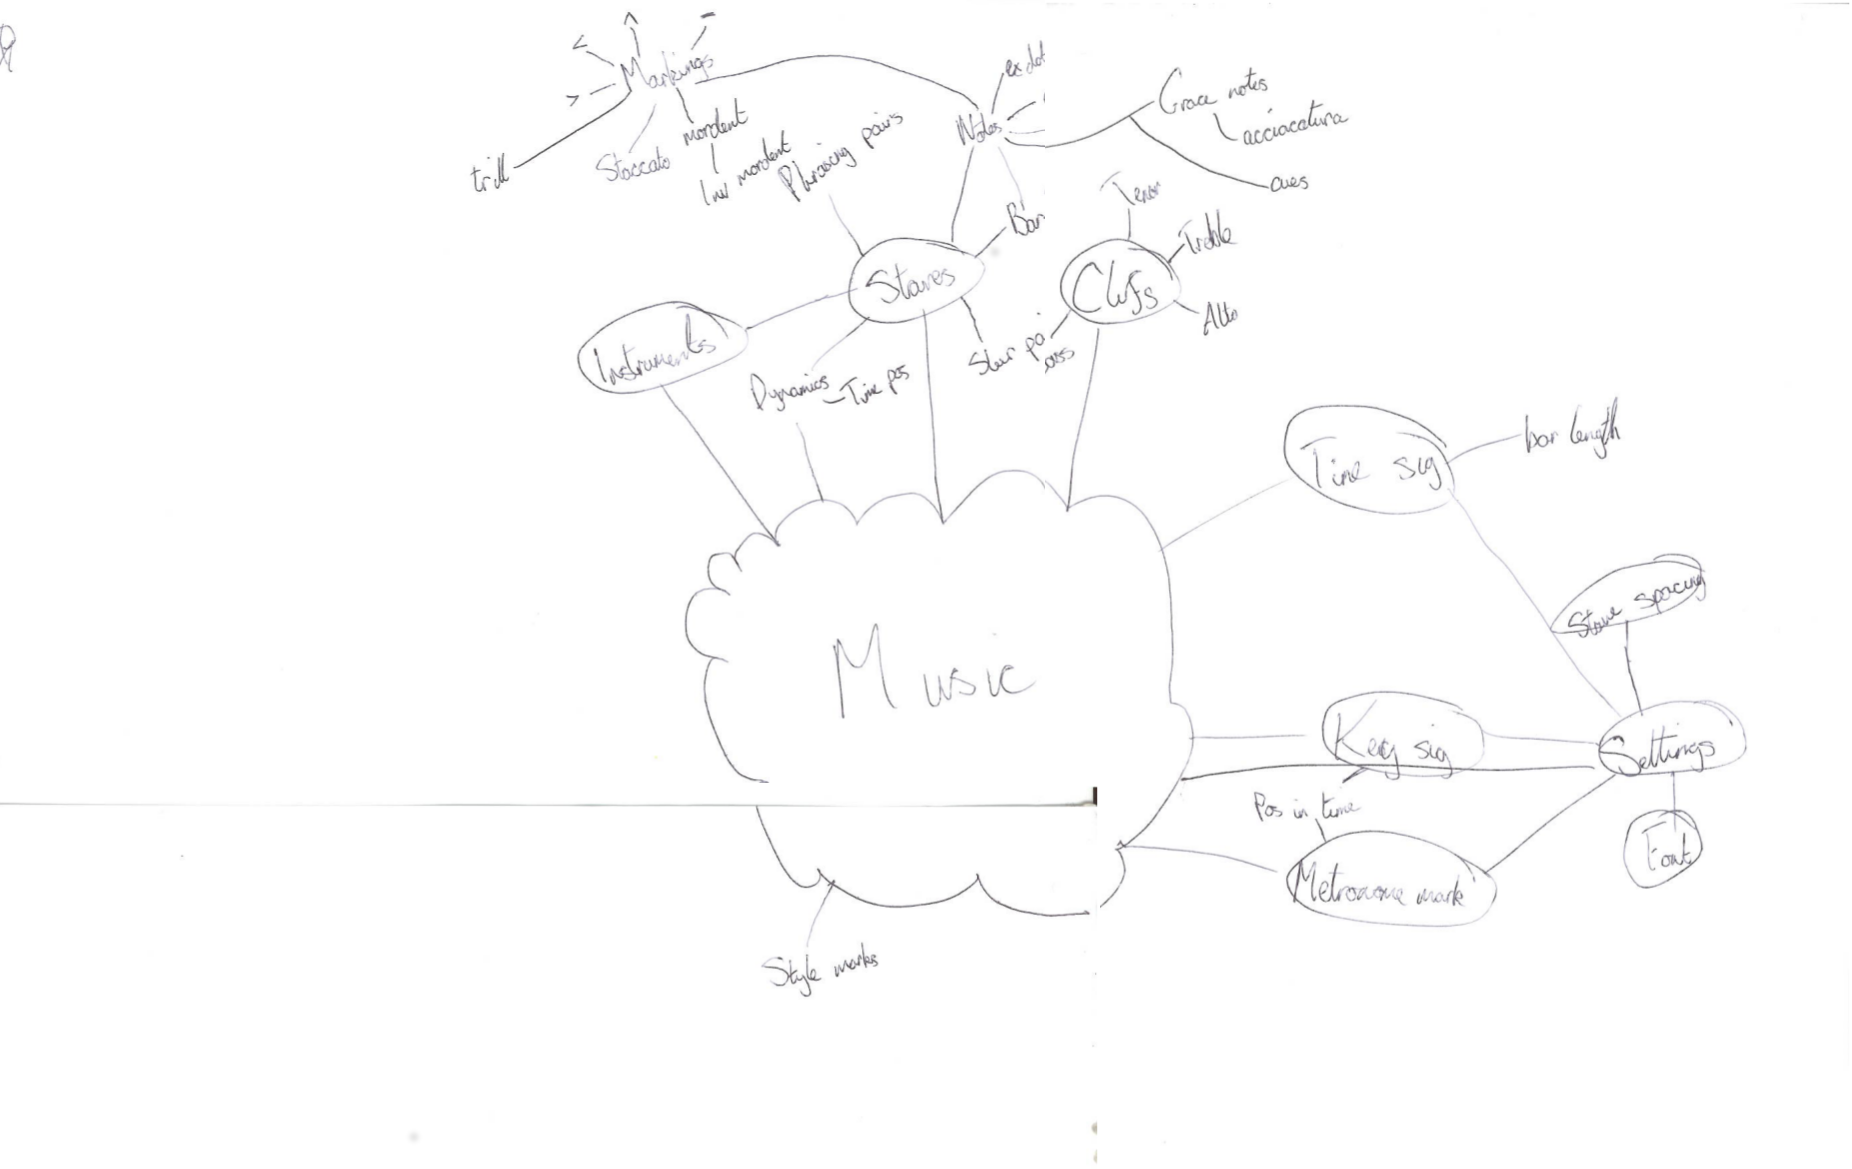
\includegraphics[width=500pt]{mindmap}
\caption{A hand drawn mindmap of elements of music}	
\end{figure}

\section{Initial class diagram}
\begin{figure}[H]
\centering
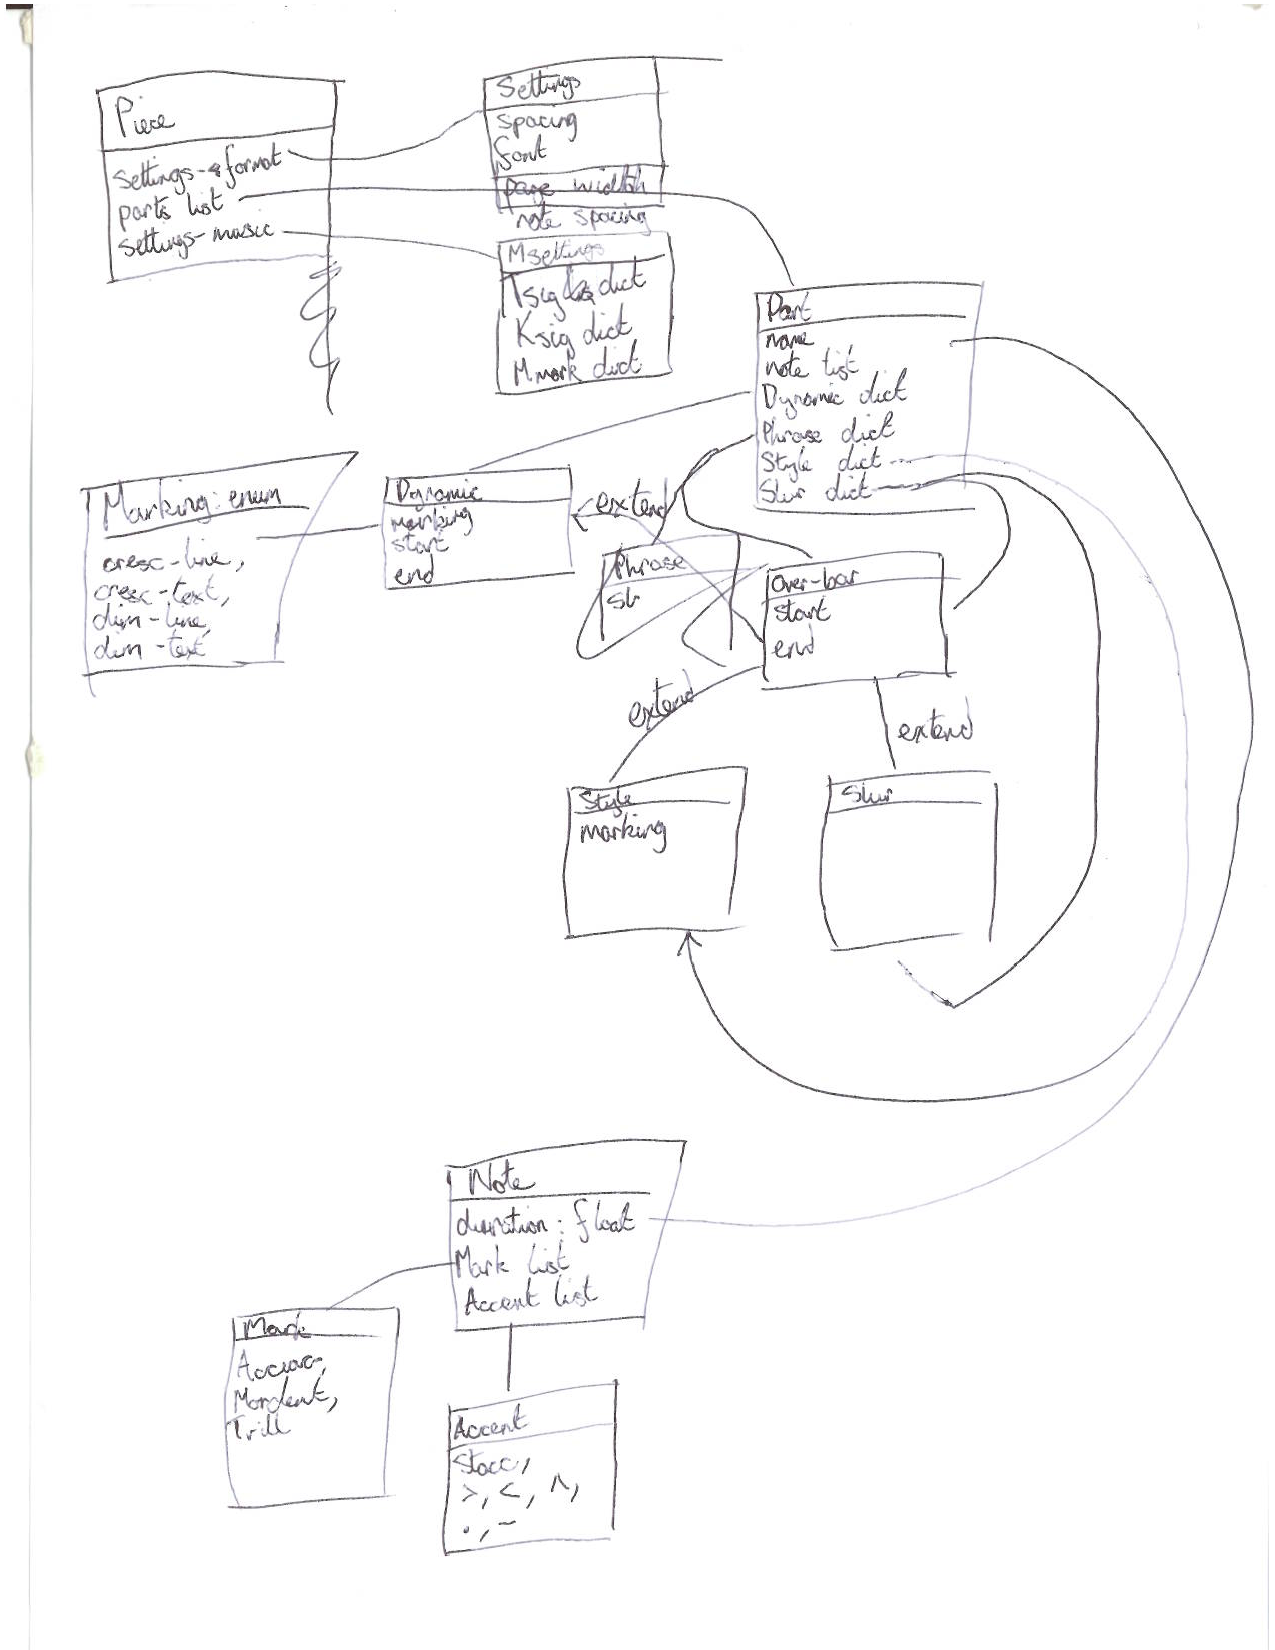
\includegraphics[width=400pt]{class-diagram}
\caption{A class diagram based on the initial mindmap}
\end{figure}
\begin{landscape}
\section{Revised computerised class diagram}
\subsection{Classes inheriting from Base}
Figure \ref{fig:base} shows all of the classes which inherit from Base. They inherit from base because the debugging "toString" method is common to all of them. Unfortunately this diagram is too big for the page.
\begin{figure}[H]
\fbox{
   \scalebox{0.4}{\includegraphics*[viewport=0 0 1750 341]{diagrams/jpegs/uml_class_diagram_for_implemen}}
  }
\caption{Classes inheriting from Base}
\end{figure}
\begin{figure}[H]
\fbox{
   \scalebox{0.4}{\includegraphics*[viewport=1750 0 3430 341]{diagrams/jpegs/uml_class_diagram_for_implemen}}
  }

\label{fig:base}
\end{figure}
\begin{figure}[H]
   \fbox{
   \scalebox{0.4}{\includegraphics*[viewport=3430 0 5100 341]{diagrams/jpegs/uml_class_diagram_for_implemen}}
   }
  
\caption{Classes inheriting from Base}
\label{fig:base}
\end{figure}
\begin{figure}[H]
   \fbox{
   \scalebox{0.4}{\includegraphics*[viewport=5100 0 5280 341]{diagrams/jpegs/uml_class_diagram_for_implemen}}
   }
  
\caption{Classes inheriting from Base}
\label{fig:base}
\end{figure}
\subsection{Notation classes}
The classes in figure \ref{fig:notation} inherit from the Notation class, for the same reasoning as those in the diagram in figure \label{fig:base} inherit from the base class. That is to say, each class has a common toString method.
\begin{figure}[h]
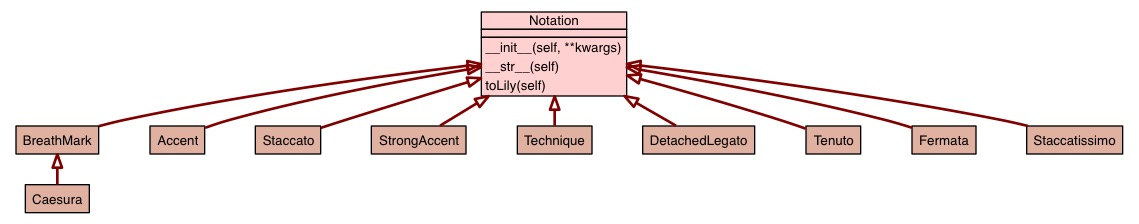
\includegraphics[width=700pt]{diagrams/jpegs/uml_class_diagram_for_implemen_34}	
\caption{Classes inheriting from Notation}
\label{fig:notation}
\end{figure}
\end{landscape}

\subsection{Exception classes}
Figures \ref{fig:mid}, \ref{fig:parterror}, \ref{fig:scorepart} are classes created to indicate to the developer that an exception has been thrown whilst parsing a musicXML file. The first indicates that no measure ID has been found, which means directions and notations cannot be added as the program does not know which measure to add them to. The second indicates that a part ID has been found which has not yet been created in the piece class when it should have, and the third indicates that no score-part ID has been found, which causes similar problems as the first exception indicates.
\begin{figure}[H]
\begin{minipage}{160pt}
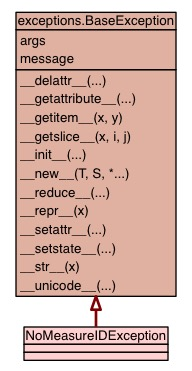
\includegraphics[width=150pt]{diagrams/jpegs/uml_class_diagram_for_implemen_19}	
\caption{MeasureID exception class}
\label{fig:mid}
\end{minipage}
\begin{minipage}{160pt}
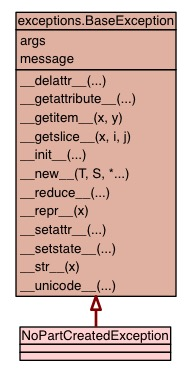
\includegraphics[width=150pt]{diagrams/jpegs/uml_class_diagram_for_implemen_20}
\caption{Part exception class}	
\label{fig:parterror}
\end{minipage}
\begin{minipage}{160pt}
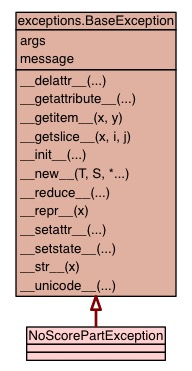
\includegraphics[width=150pt]{diagrams/jpegs/uml_class_diagram_for_implemen_21}	
\caption{ScorePart exception class}
\label{fig:scorepart}
\end{minipage}
\end{figure}
\subsection{Standalone classes}
Figures \ref{fig:clefclass}, \ref{fig:keyclass}, \ref{fig:meterclass}, \ref{fig:mxmlparse}, \ref{fig:partclass}, and \ref{fig:piececlass} do not use inheritance, as their string methods and toLily methods have no connection or similarity to any other class in the system.
\begin{figure}[H]
\begin{minipage}{160pt}
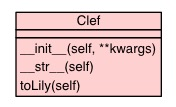
\includegraphics[width=140pt]{diagrams/jpegs/uml_class_diagram_for_implemen_2}
\caption{Clef class}
\label{fig:clefclass}
\end{minipage}	
\begin{minipage}{160pt}
	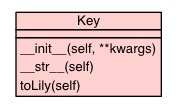
\includegraphics[width=140pt]{diagrams/jpegs/uml_class_diagram_for_implemen_28}
	\caption{Key class}
	\label{fig:keyclass}
\end{minipage}
\begin{minipage}{160pt}
	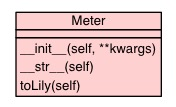
\includegraphics[width=140pt]{diagrams/jpegs/uml_class_diagram_for_implemen_45}
	\caption{Meter class}
	\label{fig:meterclass}
\end{minipage}
\begin{minipage}{160pt}
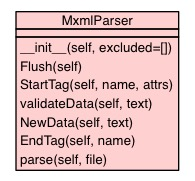
\includegraphics[width=140pt]{diagrams/jpegs/uml_class_diagram_for_implemen_46}	
\caption{The main MxmlParser class, which applies handlers to each tag}
\label{fig:mxmlparse}
\end{minipage}
\begin{minipage}{160pt}
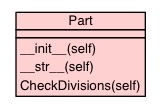
\includegraphics[width=140pt]{diagrams/jpegs/uml_class_diagram_for_implemen_66}	
\caption{Part class, which contains measures}
\label{fig:partclass}
\end{minipage}
\begin{minipage}{160pt}
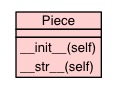
\includegraphics[width=140pt]{diagrams/jpegs/uml_class_diagram_for_implemen_67}	
\caption{Piece class, which contains parts}
\label{fig:piececlass}
\end{minipage}
\end{figure}
\section{Initial User Interface Design}
\begin{figure}[Hz]
	\centering
	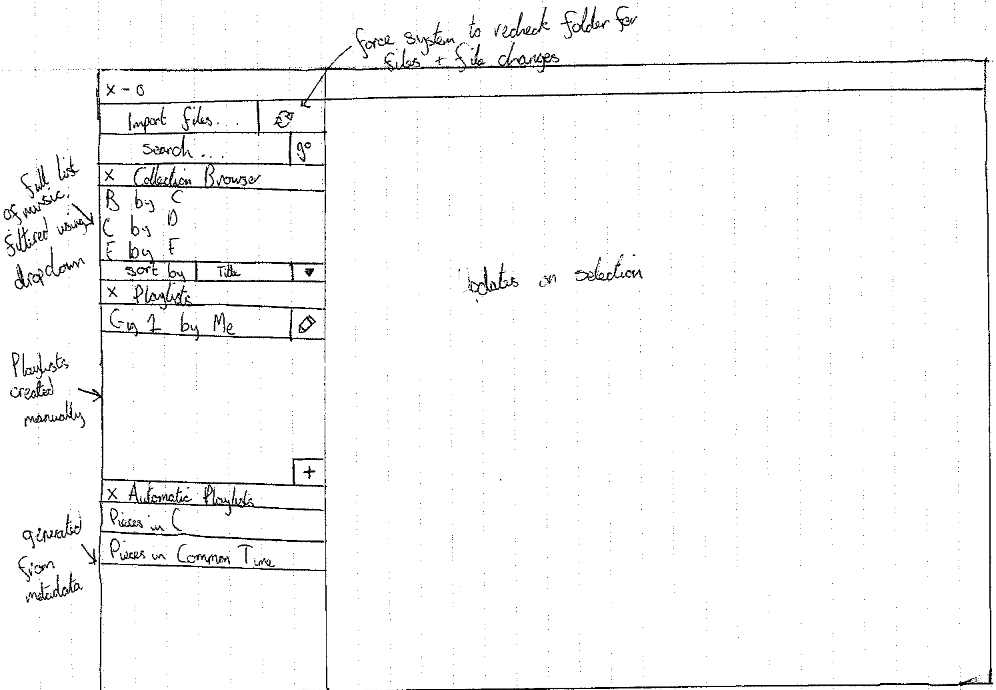
\includegraphics[width=400pt]{designs/main}
	\caption{The main GUI}
	\label{fig:m}	
\end{figure}

Figure ~\ref{fig:m} shows the main graphical user interface. Figure ~\ref{fig:import} shows the popup window displayed when "import files" is clicked. Figure ~\ref{fig:plus} shows the popup window displayed when the plus button on the playlists pane is clicked.
\begin{figure}[H]
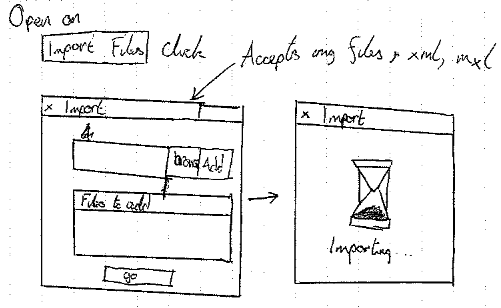
\includegraphics{designs/import_files}
\caption[width=120pt]{Popup box that opens when the user clicks "import files"}	
\label{fig:import}
\end{figure}
\begin{figure}[H]
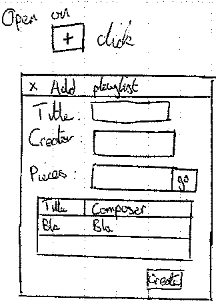
\includegraphics[width=120pt]{designs/create_playlist}
\caption{Popup box on click of the plus button, creating a new playlist}	
\label{fig:plus}
\end{figure}

\subsection{Changes to main display when sheet music selected}
\begin{figure}[H]
	\centering
	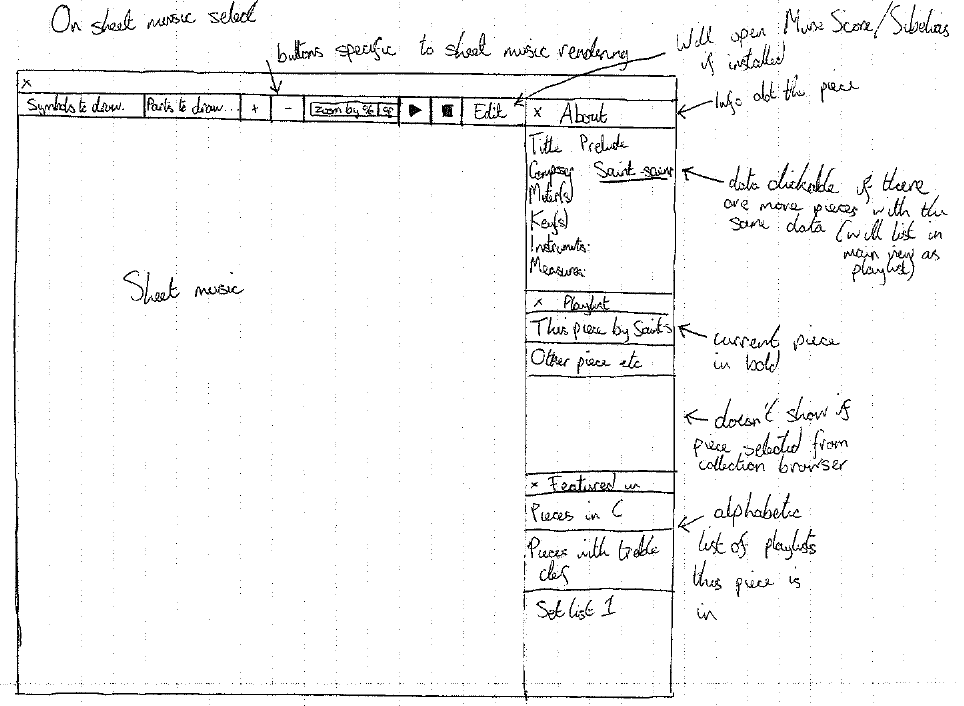
\includegraphics[width=400pt]{designs/sheet_music}
	\caption{The main pane when sheet music is selected}
	\label{fig:sheet}	
\end{figure}
The image shown in figure ~\ref{fig:sheet} shows the updated main pane of figure ~\ref{fig:m} when a piece of music has been selected. The smaller windows to the right show an about pane, which displays all information about the piece itself, a "featured in" pane which will list all playlists containing this piece, and a "playlist" pane. 

Within the about pane, if a piece of data such as "Saint-Saens" in figure ~~\ref{fig:sheet} is underlined, it can be clicked which will lead to a playlist of other pieces which contain the same data.

The playlist pane will only display if the piece has been selected for viewing from an existing playlist. That is to say, if this piece were to be clicked from the collection browser shown in figure \ref{fig:m}, this window would not be open.

\begin{figure}[H]
\begin{minipage}{160pt}
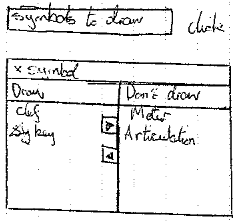
\includegraphics[width=150pt]{designs/symbol_draw}
\caption{The pop up pane displayed when symbols to draw is clicked}	
\label{fig:symbols}
\end{minipage}
\begin{minipage}{160pt}
\centering
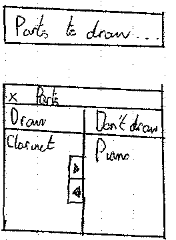
\includegraphics[width=150pt]{designs/part_draw}
\caption{the popup pain displayed when parts to draw is clicked}	
\label{fig:parts}
\end{minipage}
\begin{minipage}{160pt}
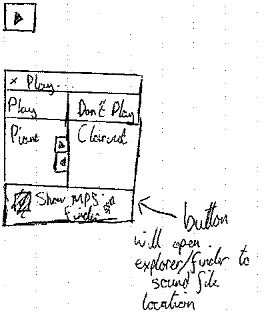
\includegraphics[width=150pt]{designs/play}
\caption{the popup pain displayed when the triangular play button is clicked}
\label{fig:play}
	
\end{minipage}
\end{figure}
The figures \ref{fig:symbols}, \ref{fig:parts}, \ref{fig:play} show the extra windows which display when "symbols to draw", "parts to draw" and the triangle (play) button are clicked, which are buttons displayed above the main pane in figure \ref{fig:sheet}. Whilst not an objective or an intended benefit, the symbols window is included in order to help users who may not be fully confident reading sheet music which includes symbols they do not understand.

\subsection{Changes to main display when playlist is selected}
\begin{figure}[H]
	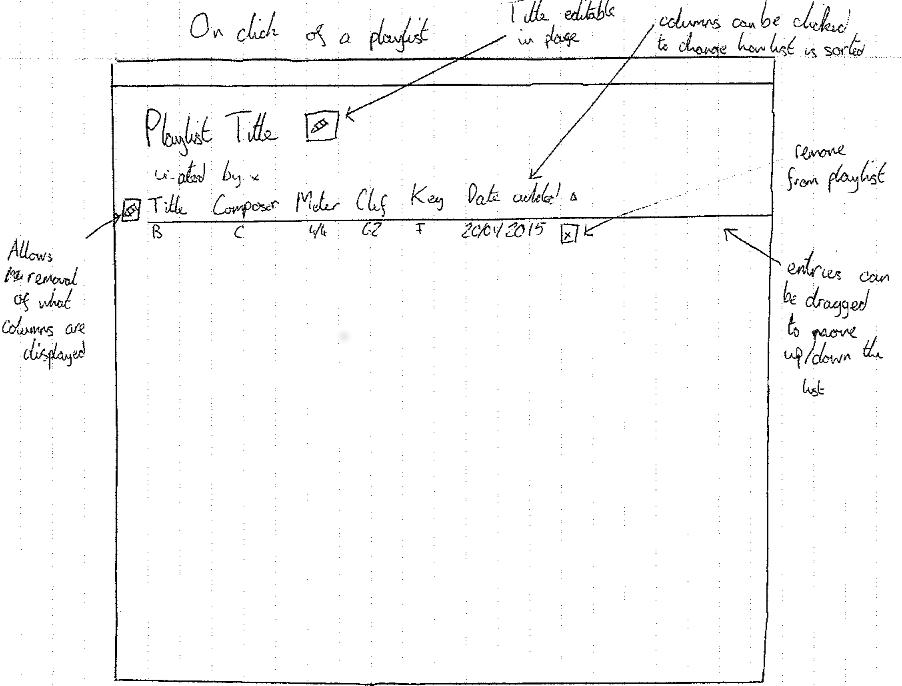
\includegraphics[width=500pt]{designs/playlist}
	\caption{The main pane of the GUI when a playlist is selected}
	\label{fig:playlist}
\end{figure}
Figure \ref{fig:playlist} shows the main pane of figure \ref{fig:m} when a playlist has been selected. This can occur by clicking a manually created playlist from the second pane in figure \ref{fig:m}, an auto-generated playlist from the third pane in the same figure, or by clicking on underlined text in the about pane of figure \ref{fig:sheet}.

The buttons which appear like pens allow the user to edit the title of the playlist or change which columns are displayed - both of these are done in place, that is to say, no extra pop up boxes are needed for the user to change anything in this window. Further to this, the user may move pieces up or down the playlist by dragging the item, and delete them using the "x" button.

\section{User Interface Feedback survey}
Figure \ref{fig:survey} shows an example blank survey given to participants to analyse the usefulness of the current user interface. This is basic, as functionality like searching at the initial survey stage will not have been connected to the user interface itself.
\begin{figure}[H]
\centering
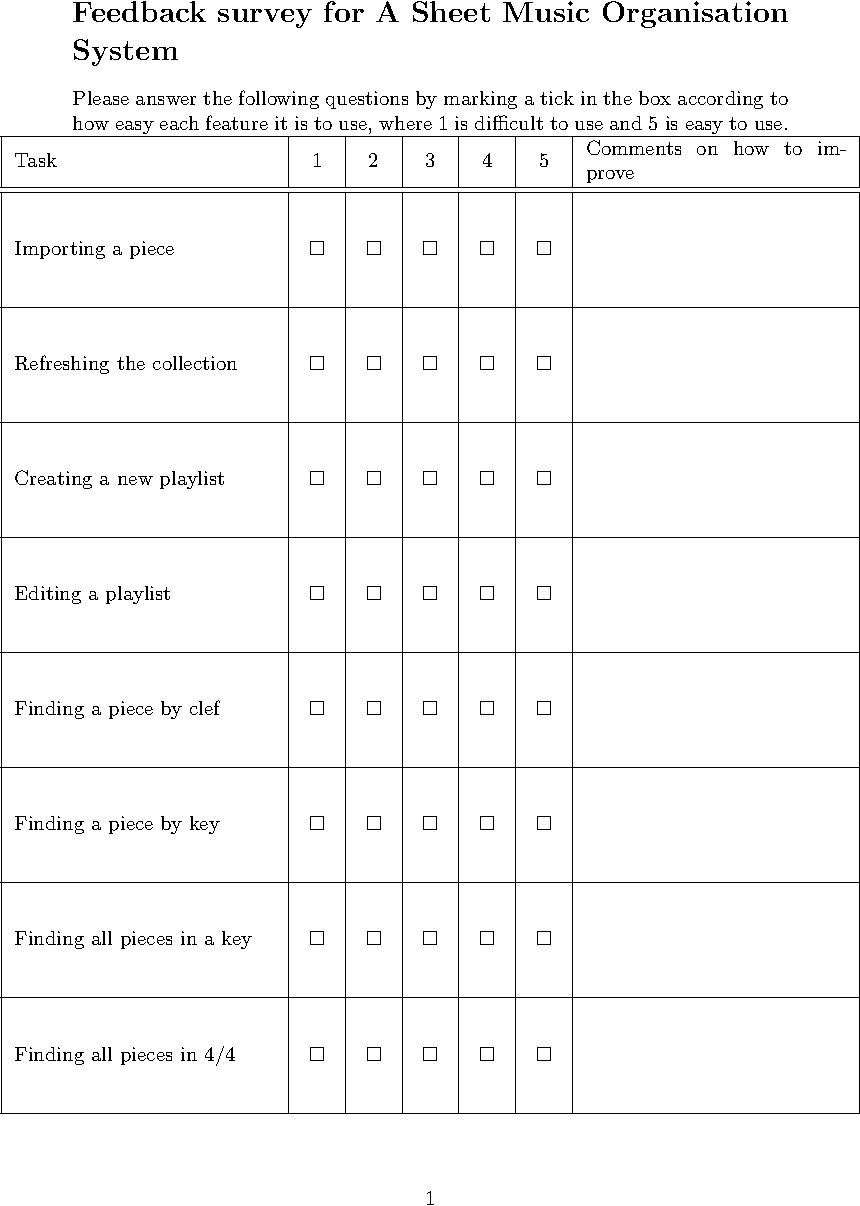
\includegraphics{survey-crop.pdf}	
\caption{The survey given to users to analyse how easy it is to use the interface}
\label{fig:survey}
\end{figure}

\section{Test list}
\section{Test cases}
Table \ref{table:testcases} gives a brief explanation of all the current testcases being used to validate the system against real world applications. Listing \ref{code:keysig} gives one example, keySignatures.xml, of a musicXML file.
\begin{table}[h]
\centering
\begin{tabu}to 1.0\textwidth{| X[l] | X[l] |} \hline
{Name} & {Purpose} \\ \hline	
Accidentals.xml & Tests system properly handles all possible accidentals attached to notes \\ \hline
GraceNotes.xml & Tests gracenotes attached to notes \\ \hline
Tremolo.xml & tests tremolo on notes \\ \hline
TrillsFermataOrnaments.xml & tests trills, fermatas (pauses) and other ornaments on notes \\ \hline
arpeggiosAndGlissandos.xml & tests arpeggios and glissandos on notes \\ \hline
barlines.xml & tests different barlines applied to measures \\ \hline
beams.xml & tests beaming of notes (quavers, semi quavers etc) \\ \hline
breathMarks.xml & tests breathmark notation next to notes \\ \hline
clefs.xml & tests all possible clef types \\ \hline
duration\_and\_stem\_direction.xml & tests duration of notes and their stem (stick) direction) \\ \hline
dynamics.xml & tests dynamics (loud and quiet) and their position in a measure \\ \hline
fingering.xml & fingering notation specific to string instruments \\ \hline
keySignatures.xml & tests all key signatures and their names are correct \\ \hline
lines.xml & tests a variety of lines over bars, such as pedal marks and repeat alternative bars \\ \hline
multiple\_parts.xml & tests how the system handles more than one instrumental part \\ \hline
noteheads.xml & tests all possible changes to the shape of the notehead \\ \hline
repeatMarks.xml & tests repeat marks are loaded correctly (i.e, points at which the player must go back to a specific sign and play it again) \\ \hline
text.xml & tests text markings, such as dynamic and tempo markings like "andante", but also things like lyrics \\ \hline
tuplets.xml & tests tuplets, where a note must be played differently to how it is notated according to it's tuplet value \\ \hline
two\_staves\_one\_part.xml & tests loading of two staves in one part, such as pianos and harpsichords \\ \hline
\end{tabu}
\caption{All testcases currently in use}	
\label{table:testcases}
\end{table}

\lstset{
    language=xml,
    tabsize=3,
    %frame=lines,
    caption=key signature testcase,
    label=code:keysig,
    frame=shadowbox,
    rulesepcolor=\color{gray},
    xleftmargin=20pt,
    framexleftmargin=15pt,
    keywordstyle=\color{blue}\bf,
    commentstyle=\color{OliveGreen},
    stringstyle=\color{red},
    numbers=left,
    numberstyle=\tiny,
    numbersep=5pt,
    breaklines=true,
    showstringspaces=false,
    basicstyle=\footnotesize,
    emph={food,name,price},emphstyle={\color{magenta}}}
    \lstinputlisting{testcases/keySignatures.xml}
\end{appendices}